\section{Кравчук Никита - Вклады в иностранные банки}
Бюджет: 100.000 евро \\

\subsection{Мотивация}
Одна из проблем, с которой столкнутся мои коллеги - конвертация денег из одной валюты в другую. В связи с этим возникла идея избежать этих расходов
и оставить деньги в евро. Так же было принято решение вкладывать деньги не в российские банки, а воспользоваться финансовыми услугами еврозоны, дабы избежать рисков, связанных с нестабильностью финансового рынка Российской Федерации. 

\subsection{Правовая основа}
Рассмотрим законы, регулирующие порядок открытия вкладов в иностранных банках для граждан Российской Федерации. Основные положения прописаны в законе №173-ФЗ «О валютном регулировании и валютном контроле»:
\\
\\
Статья 12. Счета резидентов в банках, расположенных за пределами территории Российской Федерации

1. Резиденты, за исключением случаев, предусмотренных Федеральным законом от 7 мая 2013 года №79-ФЗ "О запрете отдельным категориям лиц открывать и иметь счета (вклады), хранить наличные денежные средства и ценности в иностранных банках, расположенных за пределами территории Российской Федерации, владеть и (или) пользоваться иностранными финансовыми инструментами", открывают без ограничений счета (вклады) в иностранной валюте и валюте Российской Федерации в банках, расположенных за пределами территории Российской Федерации.

2. За исключением случаев, установленных частью 8 настоящей статьи, резиденты обязаны уведомлять налоговые органы по месту своего учета об открытии (закрытии) счетов (вкладов) и об изменении реквизитов счетов (вкладов), указанных в части 1 настоящей статьи, не позднее одного месяца со дня соответственно открытия (закрытия) или изменения реквизитов таких счетов (вкладов) в банках, расположенных за пределами территории Российской Федерации, по форме, утвержденной федеральным органом исполнительной власти, уполномоченным по контролю и надзору в области налогов и сборов.
\\
\\
Закон №79-ФЗ относится в основном к госслужащим и никакого отношения ко мне не имеет, поэтому никаких правовых препятствий со стороны законодательства РФ нет.

\subsection{Выбор страны}
Рассмотрим несколько вариантов:

\subsubsection{Швейцария}
Наверняка у большинства людей европейские банки ассоциируются именно с этой страной. Рассмотрим три крупнейших банка:

\begin{center}
	\begin{tabular}{ | l | l |}
		\hline
		Название & Процентная ставка \\ \hline
		UBS & 0.0\% \\ \hline
		Credit Suisse & 0.01-0.05\% \\ \hline
		SNB & -0.75\% \\ \hline
	\end{tabular}
\end{center}

Даже несмотря на то, что обслуживание вкладов в этих банках бесплано, вклады не смогут покрыть даже минимальную инффляцию.

\subsubsection{Ситуация в целом}
Воспользуемся агрегатором процентных ставок по депозитам в Европе:

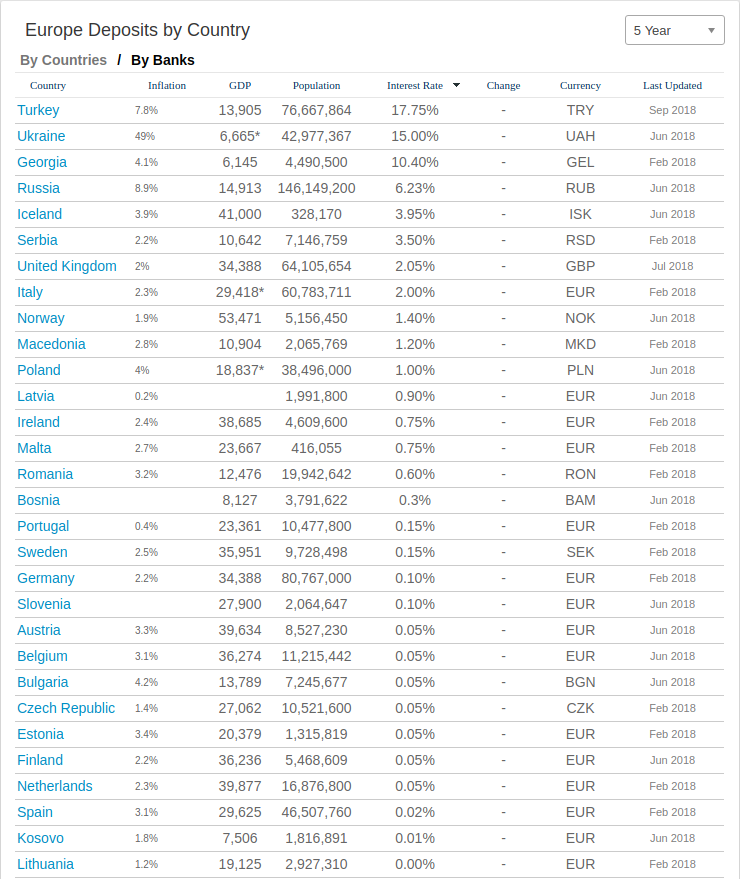
\includegraphics[width=16cm]{pics/nikita/europ.png}

Как видно из таблицы, самую большую разницу между прибылью и инфляцией можно достичь в Латвии. Рассмотрим банки этой страны.

\subsubsection{Латвия}
Рассмотрим самые доходные банки Латвии:
\\
\\

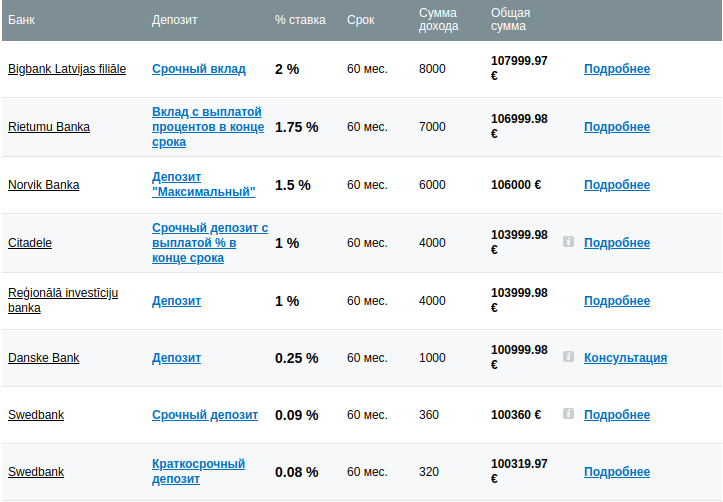
\includegraphics[width=16cm]{pics/nikita/latvia.png}

\subsection{Риски}
Европейское законодательство гарантирует возмещение средств вклада в размере до 100000 евро. Таким образом, класть всю сумму в один банк не целесообразно, поэтому воспользуемся услугами двух самых доходных банков, разделив сумму относительно их процентных ставок.

\subsection{Транспортные издержки}
Поездка в Ригу с учетом перелёта, проживания и визы обойдется примерно в 250 евро. Пренебрегая инфляцией (или отказавшись от ужина в дорогом ресторане) будем считать, что поездка спустя пять лет обойдется во столько же.

\subsection{Итог}
В итоге я открыл депозит на 53000 евро в банке Bigbank под 1.95\% и на 47000 в Rietumu Banka под 1.75\%. Спустя пят лет с учётом издержек моя сумма составит $51169.6 + 58167.5 - 500 = 108837.1$

 

